\section{System Overview}
\label{sec:systemoverview}
We introduced a location based evolving passwords scheme into the 802.11i protocol with pre-shared key mode to provide fine-grained access control and high security for WLAN. But just as significantly, introducing of evolving passwords scheme will not put extra burdens on administrators and users. To join WLAN, mobile devices must share the same password with APs at the same time, or they cannot pass APs’ authentication. However, we make passwords evolve at short intervals. A long random number is used to generate the updated password. It is called physical parameter because it can only be obtained in a constrained location protected by physical access controls for mobile devices. Once APs update their passwords, mobile devices have to  synchronize their own passwords with APs’ to join WLAN.


As is shown in Figure~\ref{fig:Overview of the WLAN System with Location Related Dynamic Password}, the location based passwords evolving system consists of three parts: a special device called physical generator which generate and broadcast physical parameters at regular intervals, one or more APs whose passwords evolve automatically at set intervals, and one or more mobile devices which are able to synchronize passwords with APs automatically when necessary and possible. 

\begin{figure}
    \centering
    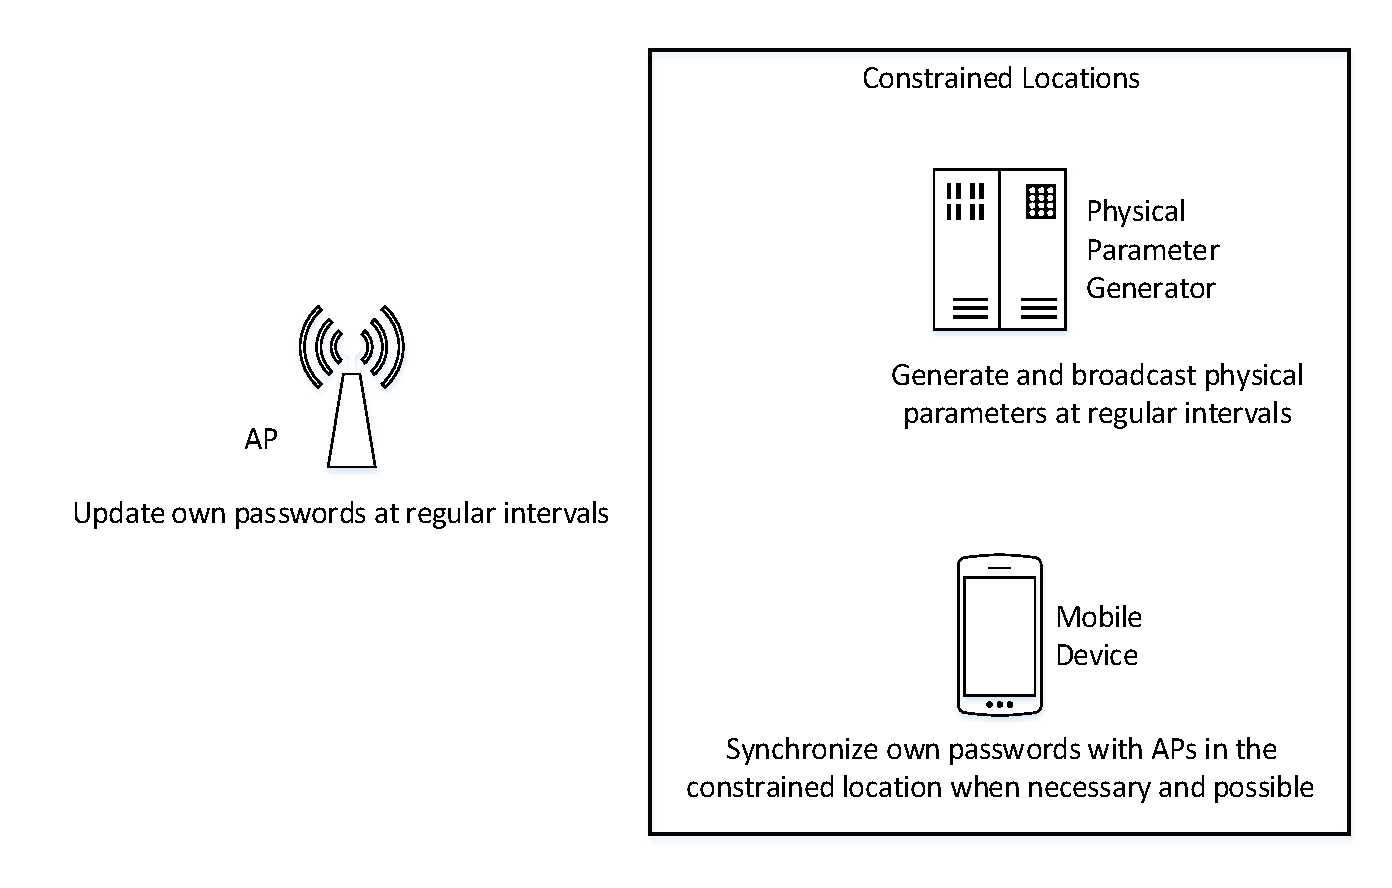
\includegraphics[width=0.5\textwidth]{pic/1.pdf}
    \caption{The WLAN System with Location Related Dynamic Password.}
    \label{fig:Overview of the WLAN System with Location Related Dynamic Password}
\end{figure}

 
\begin{itemize}
    \item the physical parameter generator will generate new physical parameters and broadcasts them to a constrained location protected by physical access controls; 
    \item APs get new physical parameters though a secure channel and update their own passwords; 
    \item  mobile devices can get new physical parameters if users pass physical access controls and update their own passwords by the same way with APs. 
\end{itemize}
	
	
APs’ initial passwords are set by administrators while mobile devices’ initial passwords are obtained through an out-of-band way. When passwords evolves, both APs and mobile devices can get the same new passwords on the basis of the same old passwords and physical parameters. The passwords evolving process is simple. The passwords evolving process of each AP and each mobile devices is independent of each other. 
